\documentclass{article}

\usepackage{hyperref}
\usepackage{listings}
\usepackage{graphicx}

\title{Semantic Enhancements for IPDL}
\author{Kristina Sojakova \and Mihai Codescu}
\date{}
\newtheorem{remark}{Remark}

\begin{document}
\maketitle
\section*{\small Acknowledgement}
This project was funded through the NGI Assure Fund, a fund established by NLnet with financial support from the European Commission's Next Generation Internet programme, under the aegis of DG Communications Networks, Content and Technology under grant agreement No. 957073.
 
\section{Omitting Arguments}

The problem has been solved by adapting the way the rules were written.
We explain this with the help of the substitution rule. The source of
the problem is Maude's treatment of variables.

The original rule for substitutions of families is (some details omitted):
\begin{lstlisting}
crl [subst-families-gen] :
 pConfig(Sigma, Delta, 
    (family (fns2[blist2]) nlist2 blist2 ::= cases) || 
    (family (fns1[blist1]) nlist1 blist1 ::=
      nf((x : T <- read (fns2[tlist]) ) BRL, R)
    ), I, O, A
 )
 => 
 pConfig(Sigma, Delta, 
   (family (fns2[blist2]) nlist2 blist2 ::= cases) || 
   (family (fns1[blist1]) nlist1 blist1 ::=
      preNF((x : T <- R2) BRL, R)
   ), I, O, A
 )
 if 
  (project2Index 
    (family (fns2[blist2]) nlist2 blist2 ::= cases) 
    nlist2 tlist A empty) 
  == 
  (fns2[tlist] ::= R2)
[nonexec] 
.
\end{lstlisting}
and since R2 does not occur in the term on the left of the equality sign
nor in the configuration that we are rewriting, the rule must be marked
as nonexecutable and R2 must be explicitly provided when the rule is applied.

The strategy $$
\mathit{substNFFamiliesGen((fam (ns1[bdlist1]), fam (ns2[bdlist2]), R)}
$$ 
that calls this rule has thus three arguments, so we can 
apply it in the strategy as 
\begin{lstlisting}
subst-families-gen[
   fns2:NameWithScripts <- ns1, 
   fns1:NameWithScripts <- ns2,
   R2:Reaction <- R
]
\end{lstlisting}

Instead of using a comparison, we have written a helper \textbf{getReaction} that gives us the reaction assigned to
\textbf{fns2[tlist]} when doing the projection, and we can use this
expression instead of R2 in the resulting pConfig. The rule is no longer
nonexecutable and we can remove the third argument of \textbf{substNFFamiliesGen}.

With this change, all substitution strategies have two arguments
and we can write a meta-strategy that handles all 
possible combinations:
\begin{lstlisting}
 strat subst : CNameBound CNameBound @ ProtocolConfig .
 sd subst(chn C1, chn C2) :=
            substNFRead(C1, C2) 
    or-else substNF(C1, C2)
 . 
 sd subst(fam (fns1[bdlist1]), fam (fns2[bdlist2])) :=
    substNFFamiliesGen(
     fam (fns1[bdlist1]), fam (fns2[bdlist2])
    )
 . 
 sd subst(fam (fns1[bdlist1]), chn C2) :=
    substNFFamilyOne(fam (fns1[bdlist1]), C2)
 .
 sd subst(chn C1, fam (fns2[bdlist2])) :=
    substChannelFamilyOne(chn C1, fam (fns2[bdlist2]))
 .
 
\end{lstlisting}
\noindent which was our original goal. 

We had a similar issue with the type of an expression/reaction.
Just like above, it can be computed and thus
eliminated as an argument of the strategy.

\section{IPDL-specific Error Handling}

We have added type checking steps in the analysis of protocols in the SpeX implementation of IPDL. We have attempted to do this in the original 
implementation, but Maude provides limited capabilities for printing
values of any type. SpeX provides an appropriate solution to this,
and we can simply reuse it. We have refactored the analysis of
protocol declarations by adding a pre-processing step that
removes the token constructors (SpeX-specific implementation detail),
followed by a type checking step that reuses the type checking already
implemented and throws an error if some condition fails to hold (this code is again written at a SpeX-specific level).
In Fig.~\ref{fig:typing} we see how
IPDL displays various error messages. Notice that now the types can be displayed instead of getting just a type assigment error, and we get a pointer to where the error happened (provided by SpeX).

\begin{figure}[htp]
\caption{Type-checking errors.}\label{fig:typing}
\centering
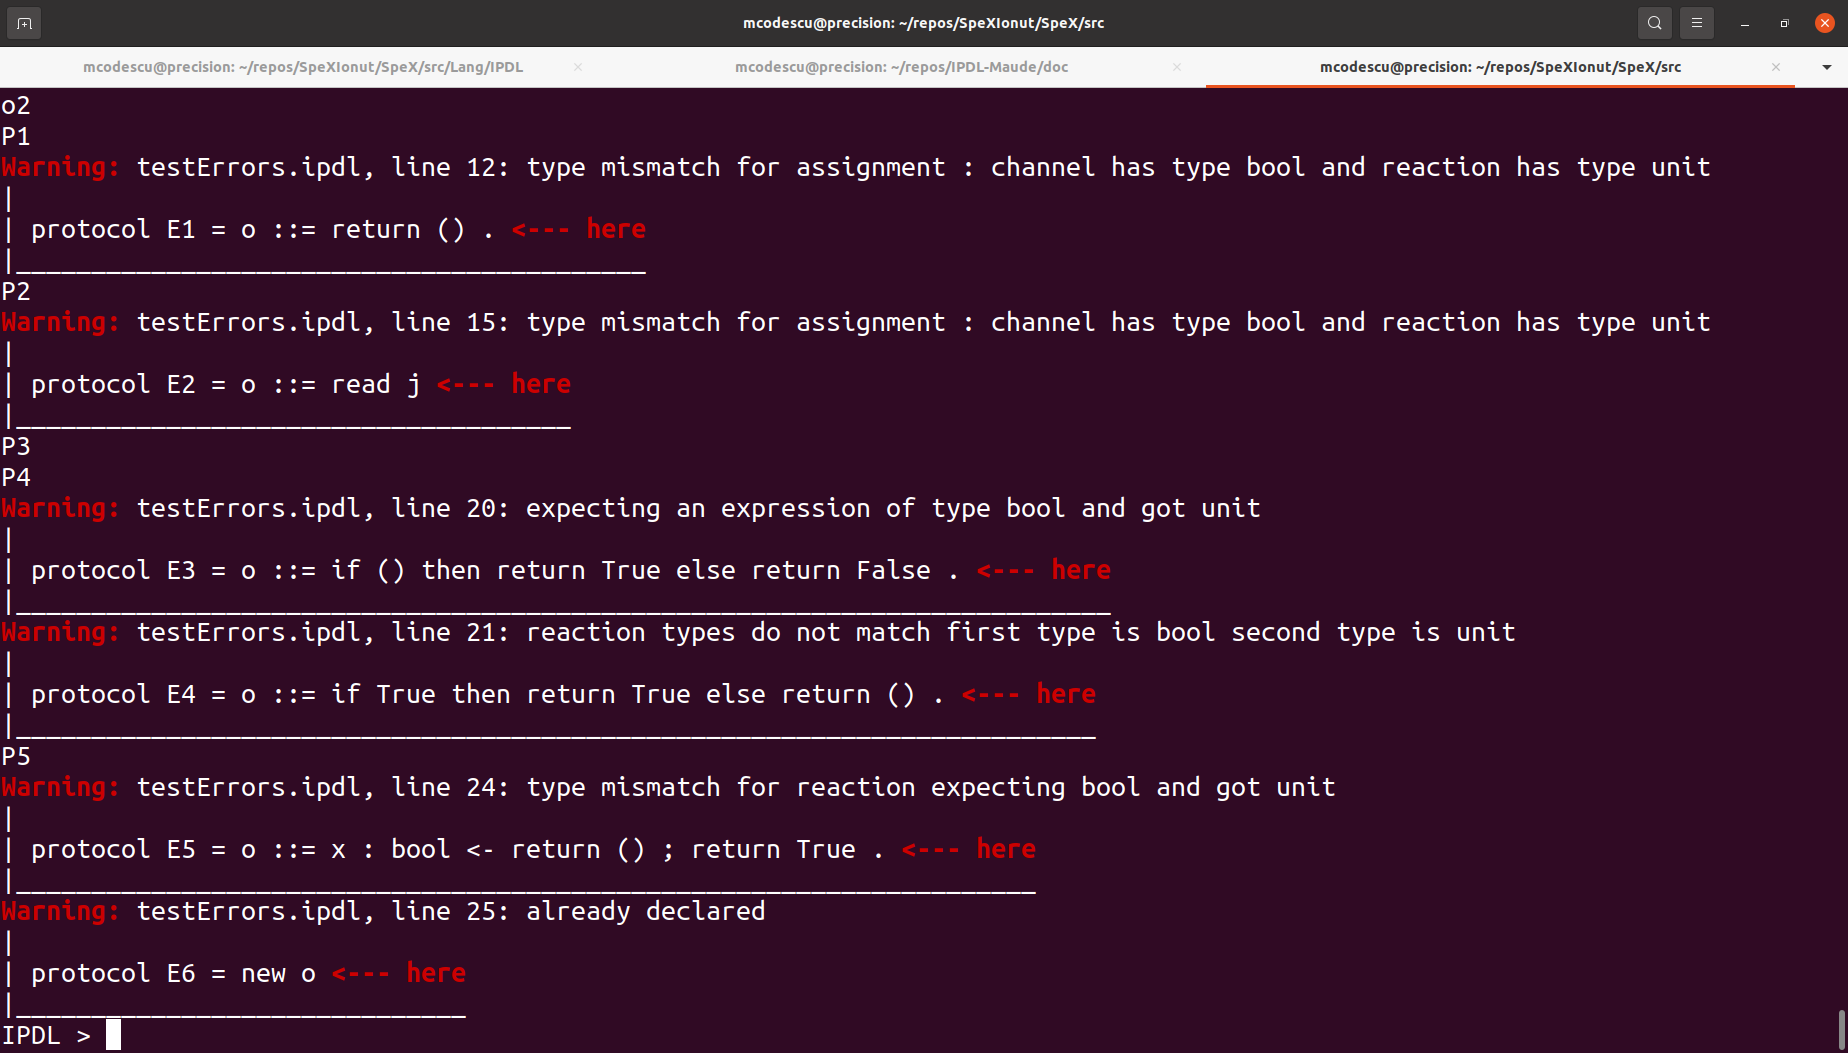
\includegraphics[width=\textwidth]{typing}
\end{figure}

We have also added some support for the case that a strategy does not
apply to the current protocol. Maude only answers this with "No solution.".
While the problem of why a rule cannot be applied to a protocol is too
complex to be solved in general, we can at least provide the left-hand side of the rule that we are trying to apply and the protocol fragment that we
are trying to apply it to, and the user can compare the two. In Fig.~\ref{fig:rule} we see the result of failing to apply a strategy to
a protocol.

\begin{figure}[htp]
\caption{Rule cannot be applied.}\label{fig:rule}
\centering
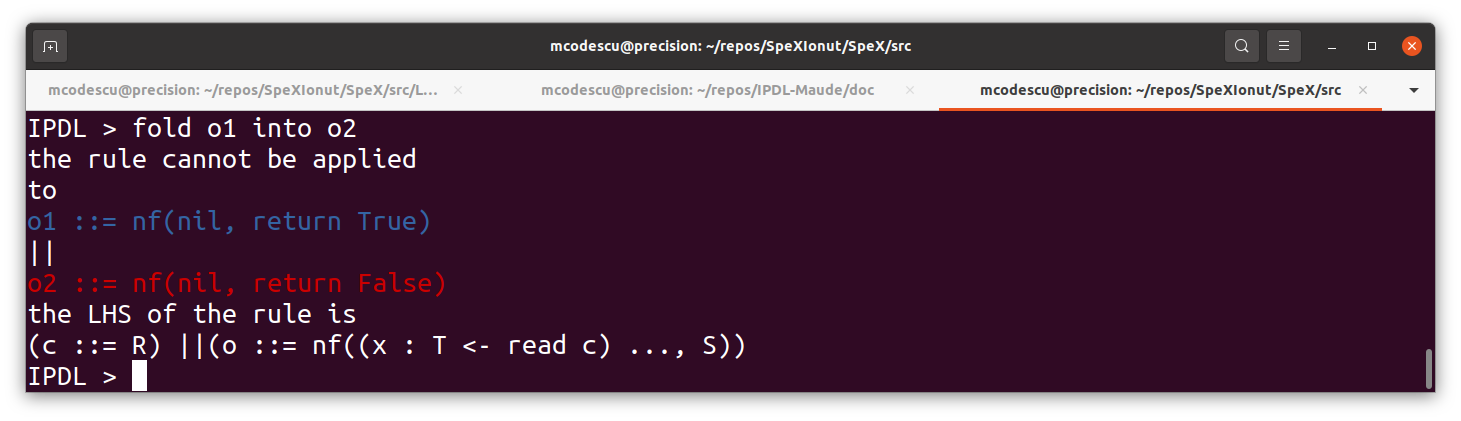
\includegraphics[width=\textwidth]{proof}
\end{figure}


\end{document}

